%! TeX encoding = UTF-8 unicode
%%%%%%%%%%%%%%%%%%%%%%%%%%%%%%%

\documentclass[10pt,aps,prb,amsmath,amssymb,twocolumn,letterpaper,nobalancelastpage,final,citeautoscript,floatfix,raggedbottom,superscriptaddress]{revtex4-1}

%%%%%%%%%%%%%%%
% MY SETTINGS
%%%%%%%%%%%%%%%v
\usepackage[usenames,dvipsnames]{color}
\usepackage{graphicx}
\usepackage{microtype}
\usepackage[bookmarks=false,colorlinks]{hyperref}
\usepackage{xfrac}
\hypersetup{
    linkcolor=RubineRed,          % color of internal links
    citecolor=ForestGreen,        % color of links to bibliography
    filecolor=Mulberry,      % color of file links
    urlcolor=RoyalBlue           % color of external links
}
\usepackage{natbib}
%additional commands
\newcommand{\textapprox}{\raisebox{0.5ex}{\texttildelow}}
\newcommand{\gvs}{GaV$_4$S$_8$}
\newcommand{\gvse}{GaV$_4$Se$_8$}
\newcommand{\gms}{GaMo$_4$S$_8$}
\newcommand{\gmse}{GaMo$_4$Se$_8$}
\newcommand{\gns}{GaNb$_4$S$_8$}
\newcommand{\gnse}{GaNb$_4$Se$_8$}
\newcommand{\gts}{GaTa$_4$S$_8$}
\newcommand{\gtse}{GaTa$_4$Se$_8$}

\newcommand{\dpg}[1]{\textcolor{red}{#1}}


%%%%%%%%%%%%%
% MAIN TEXT
%%%%%%%%%%%%%

\begin{document}

\title{Analysis of alloy steel composition-property \\ relationship using machine learning}

\author{Raymond Wang}
  \affiliation{Department of Materials Science and Engineering, Northwestern University, Evanston, Illinois  60208, USA}

  
%%%%%%%%%%%%%
% ABSTRACT
%%%%%%%%%%%%%

\begin{abstract}
This challenge project obtains digital alloy steel data from online resources and then converts them into machine-readable format. Data analysis using correlation heatmap shows degree of correlation within alloy steel composition and properties. Several strongly correlated quantities (e.g. hardness and tensile strength) are identified. Machine learning algorithm performance on predicting composition-property relationship is benchmarked using grid search. XGBoost outperforms the other methods in this case. Further analysis shows predicting thermal conductivity from chemical composition using XGBoost has satisfying accuracy and the model performance can be improved by having more training data. Our findings suggest that machine learning methods could provide more insights of alloy steel composition-property relationship than using human intuition or experience.
\end{abstract}

\maketitle

%%%%%%%%%%%%%%%%%%%%%%%%%%%%%%%%%%%%%%
% MOTIVATION
%%%%%%%%%%%%%%%%%%%%%%%%%%%%%%%%%%%%%%

\section{Workflow}

This challenge project mainly consists of five sections, i.e. data acquisition, featurization, human interpretation, machine learning model training, and results analysis. The flowchart and specific outcomes in each step are shown in Figure \ref{fig:flowchart}. The rest of this report will span these five sections into details of implementation and obtained results. Data is available at the author's \href{https://github.com/raymond931118/scraping}{GitHub}, the code can be found in supporting information (SI).

\begin{figure}[h]
  \center
  \vspace{-1mm}
 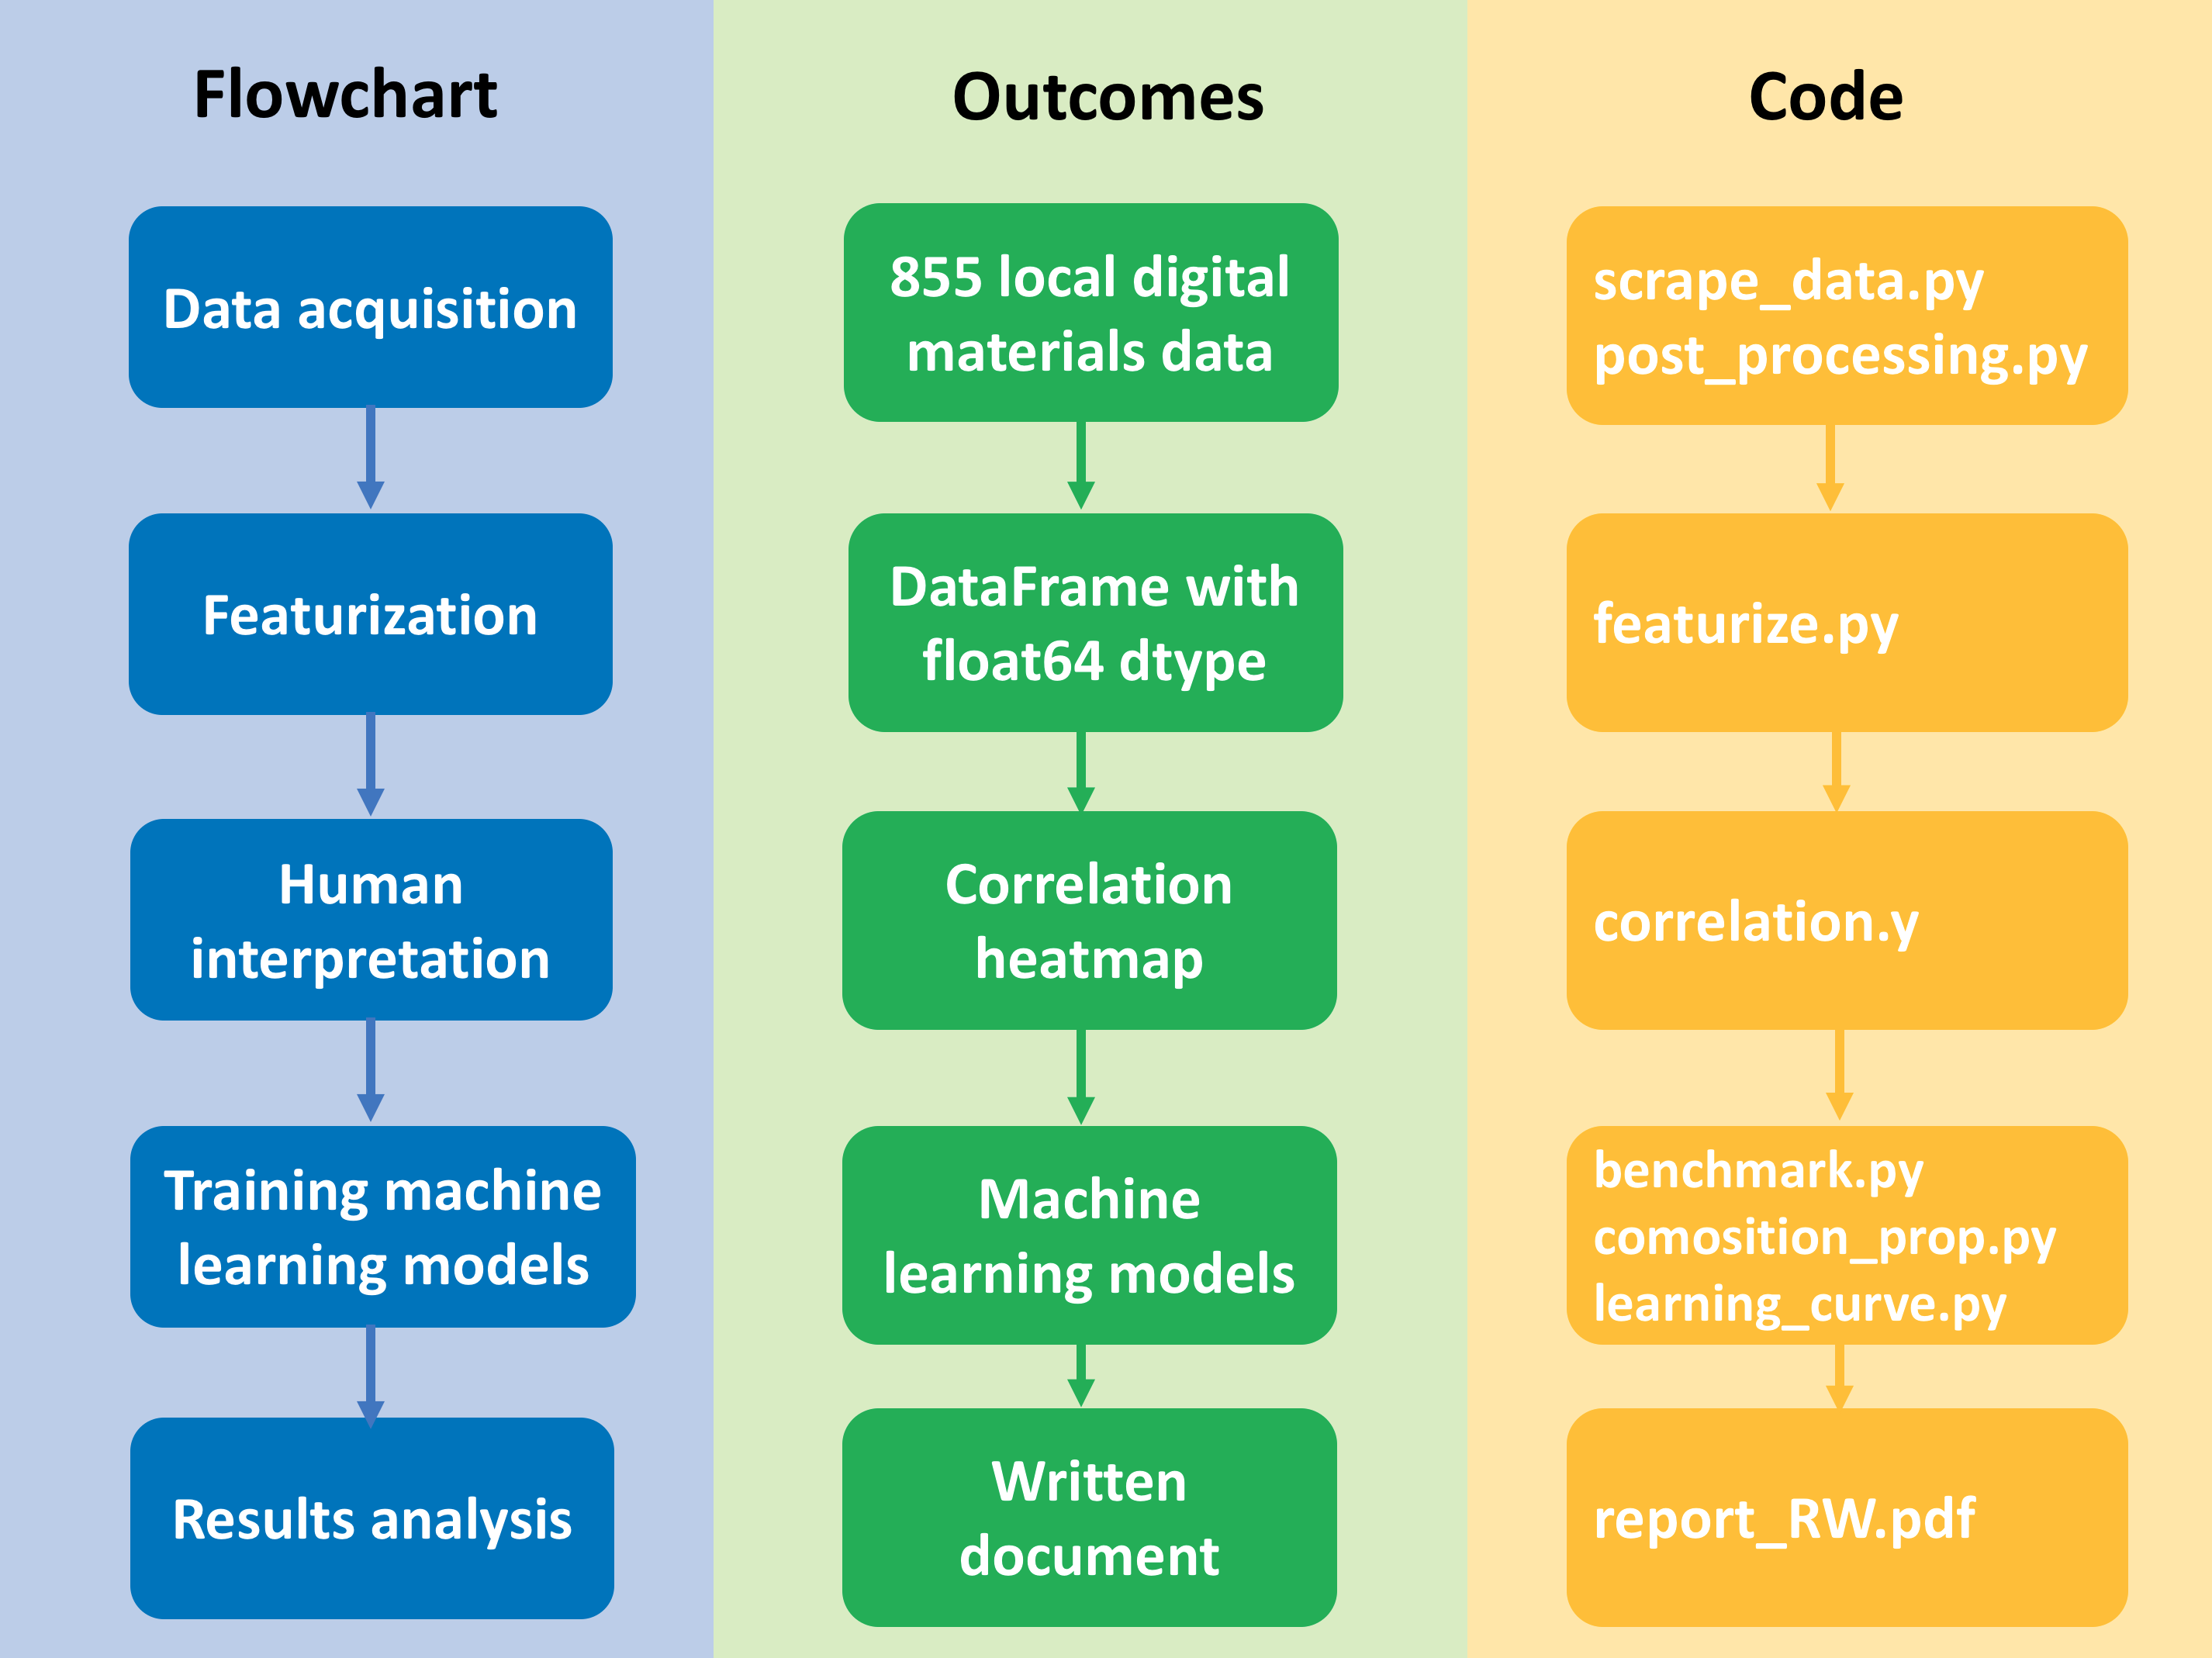
\includegraphics[width=0.95\linewidth]{figures/flowchart.png}
  \caption{Flowchart of the challenge project.}
  \label{fig:flowchart}
\end{figure}




%%%%%%%%%%%%%%%%%%%%%%%%%%%%%%%%%%%%%%
% DATA ACQUISITION
%%%%%%%%%%%%%%%%%%%%%%%%%%%%%%%%%%%%%%
\section{data acquisition}

The challenge project starts from acquiring materials data from online resources. Automated scraping code is developed by the author in Python, which automatically collects materials information that meets the searching criteria and saves to local CSV files.d by the author. 

Materials data is collected from \href{http://www.matweb.com/index.aspx}{MatWeb}, where alloy steels containing Manganese, Chromium, and Nickel are set as the target materials for scraping. Each entry of material data spans four columns and multiple rows, as shown in Table \ref{tab:web_data}. Data under `English' has different unit from `Metric', this project only processes data with metric unit.

\vspace{-10pt}
\begin{table}[h]
\begin{ruledtabular}
\caption{Format of online resources.\label{tab:web_data}}\centering
\begin{tabular}{llll}
\sffamily Property & \sffamily Metric & \sffamily English &  \sffamily Comments \\
\hline 
Elongation at break & 55\% & 55\% & some comments \\
\hline
$\cdots$ & $\cdots$ & $\cdots$ & $\cdots$
\end{tabular}
\end{ruledtabular}
\end{table}

Both physical properties (e.g. Bulk modulus, thermal conductivity) and chemical compositions (e.g. weight of Mn, Ni, Cr) in different units, as well as the potentially helpful comments, are saved to local files with the same format. Since there is no data-editing related in this step, the local data is guaranteed to be the same as its online version.

One of the technical challenges during data acquisition is IP-blocking from the server. MatWeb will block the IP (possibly permanently) once it detects over access within a short period of time. From the author's experience, one IP address gives access to 100$\sim$200 materials information per day. One of the advantage of the developed code is its high portability. The only two dependencies are \texttt{selenium} and \texttt{pandas} packages, which can be installed easily. In order to accelerate the project, the author used six machines with Unix-like systems for development and production. Eventually the program extracted 855 alloy steels that meet the criteria. The code (\texttt{scrape.py}) is available in SI.

Simple post-processing is performed right after all the data has been saved locally. This step modifies the file names and contents containing non-utf-8 encoding and fixes unwanted line breaks. The process file is still string-based, relevant code is available is SI (\texttt{post\_processing.py}).

%%%%%%%%%%%%%%%%%%%%%%%%%%%%%%%%%%%%%%
% FEATURIZATION
%%%%%%%%%%%%%%%%%%%%%%%%%%%%%%%%%%%%%%
\section{featurization}

The data collected from the last step is still string-based, e.g. ``97\%'' is interpreted as a combination of characters instead of a floating point number. Therefore, it is necessary to convert these strings to machine-readable form before any further data analysis.

Since there are multiple materials properties and not all of them are available for each materials, dataset with missing values will be dropped. In order to keep a relatively large number of training set, we only converted physical properties with more than 100 available measured data points. These physical variables are: density, hardness (Vickers), thermal conductivity, specific heat capacity, CTE-linear, electrical resistivity, elongation at break, bulk modulus, modulus of elasticity, shear modulus, poisson's ratio, tensile strength at yield, and tensile strength at ultimate. Ten element types including Fe, Mn, Cr, Ni, Mo, Cu, C, S, Si, P are considered.

Floating point numbers are extracted from string data and converted to \texttt{pandas.DataFrame} format. The converted dataset is shown in Table \ref{tab:featurization}. Non-available data points are converted to \texttt{nan} instead of `N/A'. The `\%' and other units are dropped, only the floating point numbers are extracted. Since data will be standardized before numerical processing, the only thing to make sure is that all data in the same column share the same unit/percentage sign. The code is available in SI (\texttt{featurize.py}).

\vspace{-10pt}
\begin{table}[h]
\begin{ruledtabular}
\caption{Format of data after featurization.\label{tab:featurization}}\centering
\begin{tabular}{ccccccc}
\sffamily Fe & \sffamily Mn & \sffamily Cr &  \sffamily $\cdots$ &  \sffamily Hardness &  \sffamily Bulk modulus &  \sffamily $\cdots$ \\
\hline 
97.16 & 0.88 & 0.5 & $\cdots$ & 220 & \texttt{nan} & $\cdots$\\
\hline
95.43 & 0.85 & 0.0 & $\cdots$ & \texttt{nan} & 160 & $\cdots$\\
\hline
$\cdots$ & $\cdots$ & $\cdots$ & $\cdots$ & $\cdots$ & $\cdots$ & $\cdots$
\end{tabular}
\end{ruledtabular}
\end{table}


%%%%%%%%%%%%%%%%%%%%%%%%%%%%%%%%%%%%%%%%%
% DATA ANALYSIS WITH HUMAN INTELLIGENCE
%%%%%%%%%%%%%%%%%%%%%%%%%%%%%%%%%%%%%%%%%
\section{data analysis with human intelligence}

The size of the dataset after featurization is 726$\times$23 (with 726 instances and 23 features). It is impractical for humans (at least for the author) to directly learn patterns from such large amount of data. Based on basic statistical knowledge, the author decides to start from learning correlation patten of these variables. The instances with \texttt{nan} entries are dropped from the dataset, and eventually 254 materials are used to generate the heatmap, which is shown in Figure \ref{fig:heatmap}. The code can be found in SI (\texttt{correlation.py})

\begin{figure*}[t]
  \center
 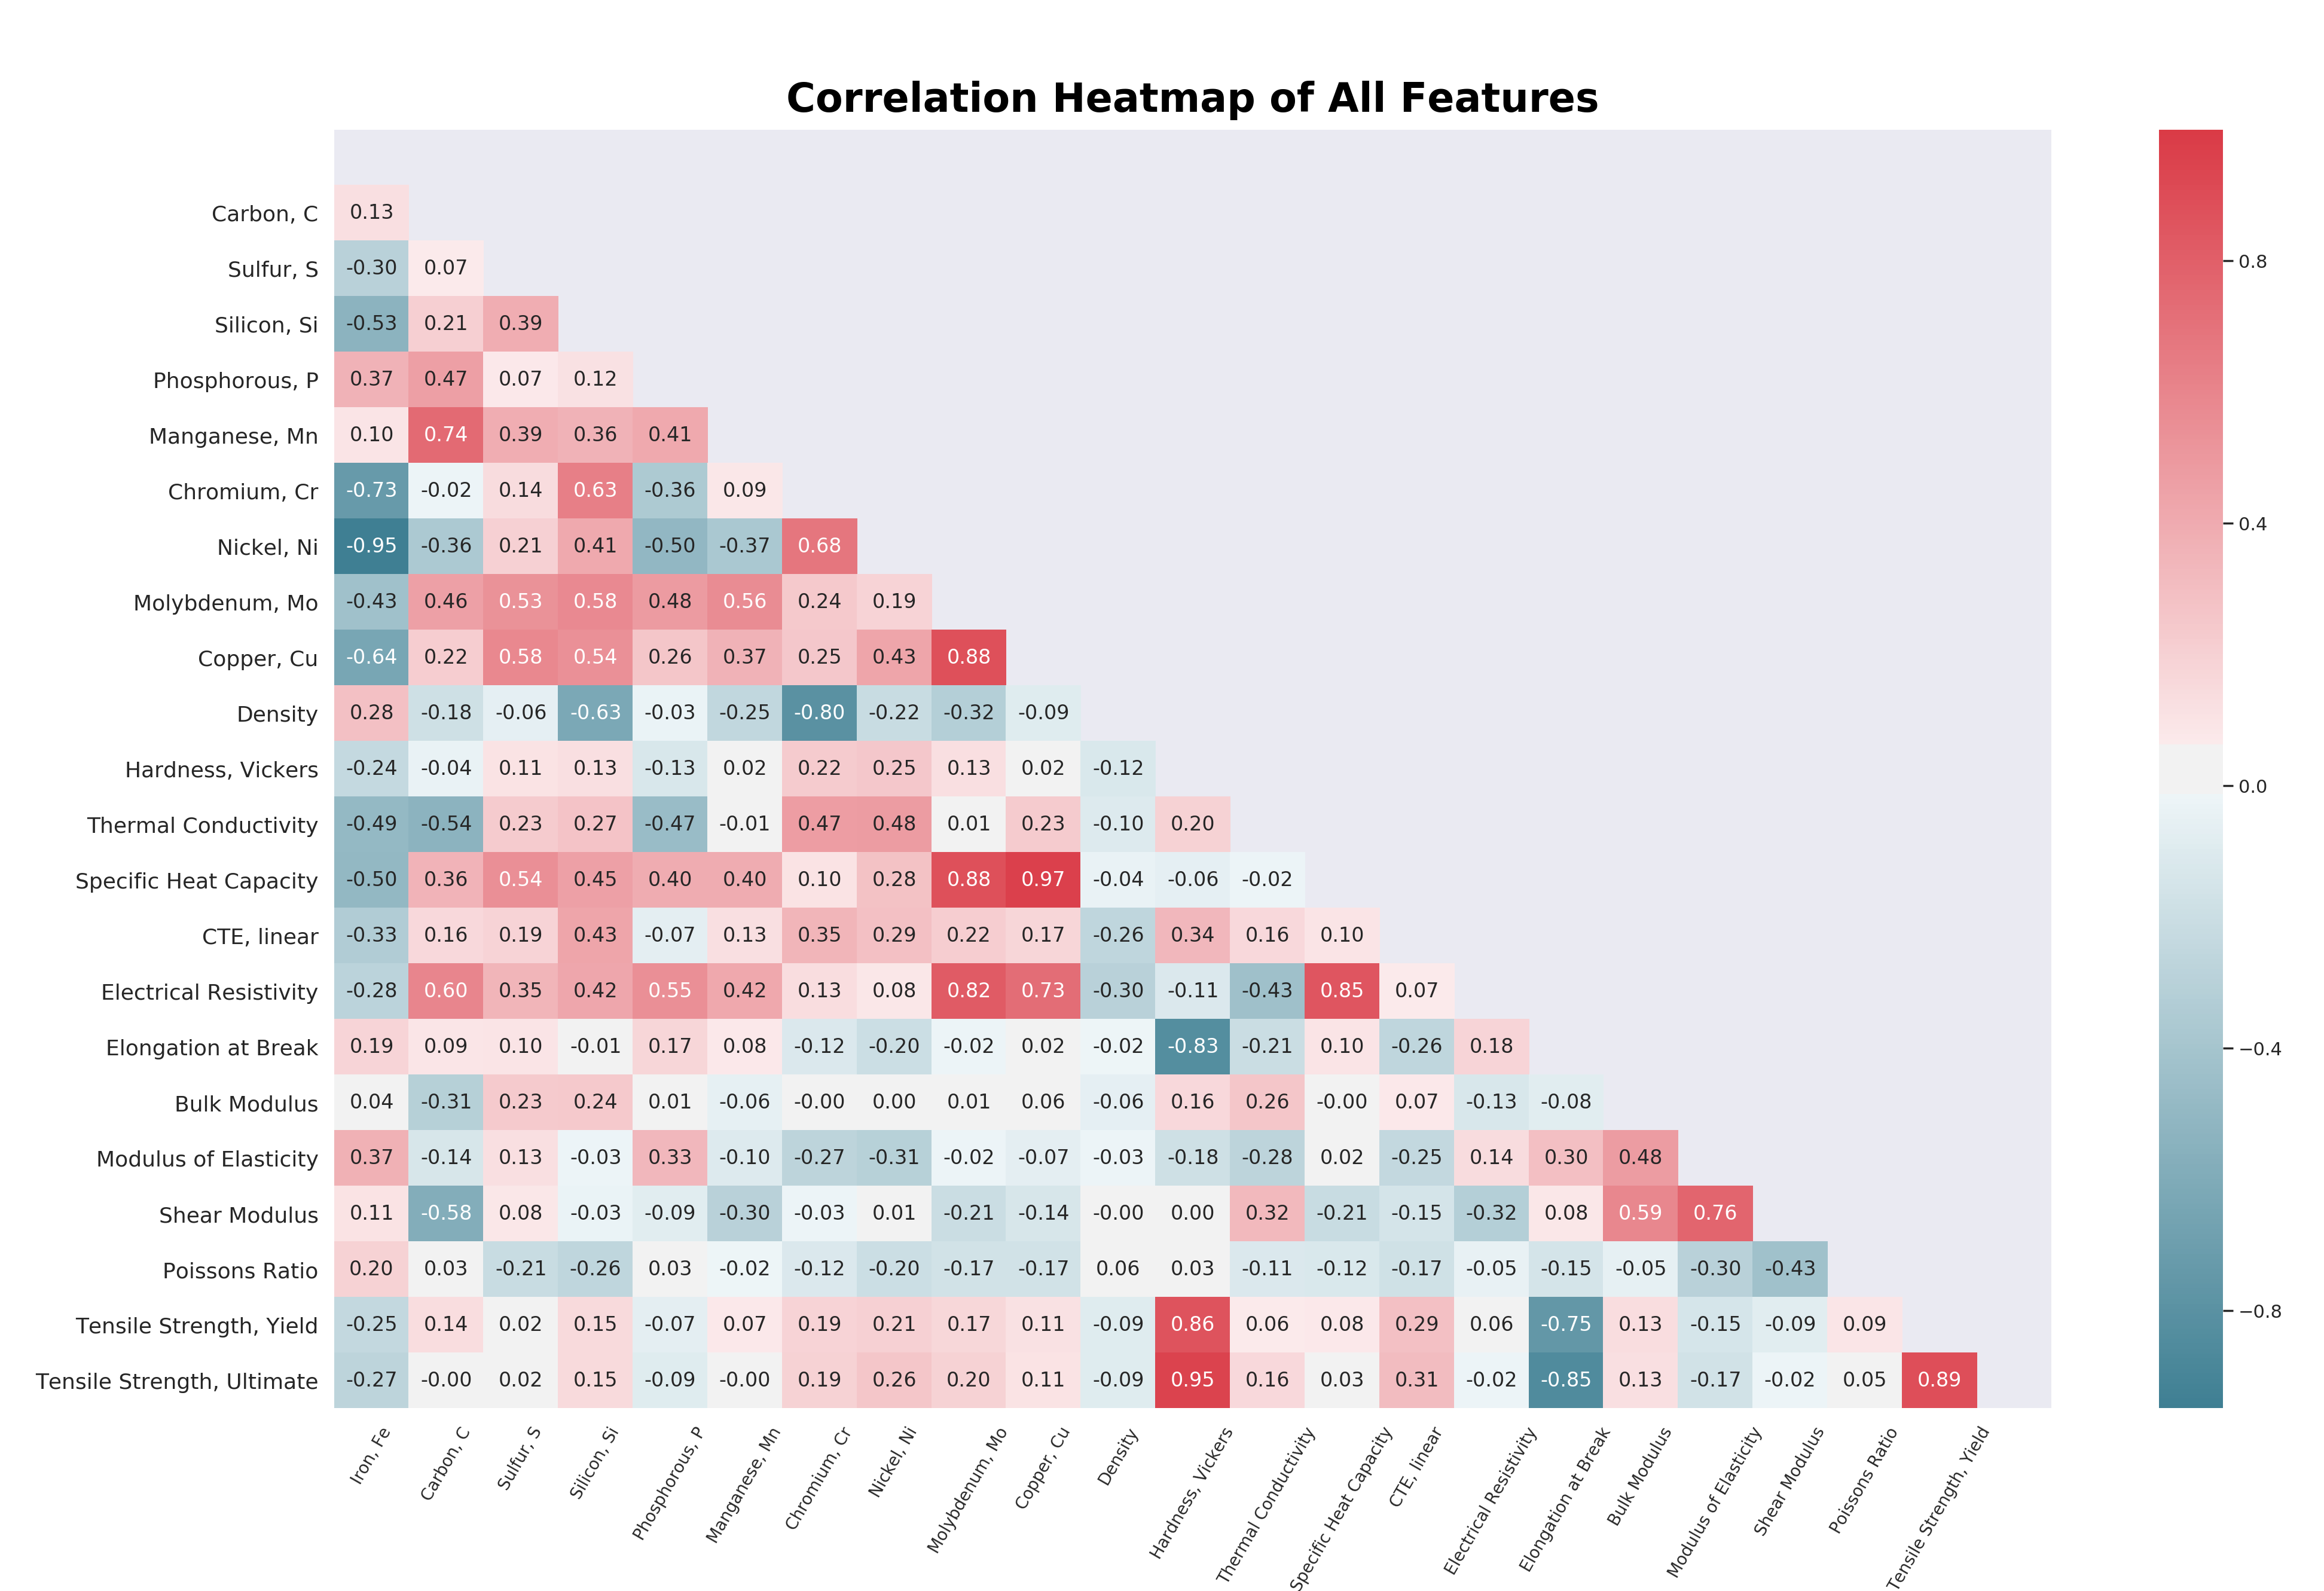
\includegraphics[width=0.85\linewidth]{figures/heatmap_mask.png}
  \caption{Correlation heatmap of chemical composition and physical properties.}
  \label{fig:heatmap}
\end{figure*}

Some of the discoveries from the heatmap include:
\begin{enumerate}
	\item[i.] Carbon increases electrical resistivity but decreases shear modulus
	\item[ii.] Sulfur increases specific heat capacity
	\item[iii.] Phosphorus increases electrical resistivity
	\item[iv.] Chromium decreases density
	\item[v.] Molybdenum and copper strongly increases specific heat capacity and electrical resistivity
	\item[vi.] Nickel increases thermal conductivity
	\item[vii.] Hardness is positively correlated to tensile strength and negatively correlated to elongation at break
	\item[viii.] Electrical resistivity is positively related to specific heat capacity
\end{enumerate}


Some of the findings agree well with the way elements contribute to alloy steel properties as reported online, e.g. carbon decreases ductility of steel, possibly could lead to a small shear modulus. However, the information from correlation analysis is more qualitative than quantitative. If we want more quantitative descriptions of the materials composition-property relationship, more sophisticated methods are needed. In the next section we discuss alloy steel data analysis using machine learning models.


%%%%%%%%%%%%%%%%%%%%%%%%%%%%%%%%%%%%%%%%%%%%%%
% DATA ANALYSIS WITH ARTIFICIAL INTELLIGENCE
%%%%%%%%%%%%%%%%%%%%%%%%%%%%%%%%%%%%%%%%%%%%%%
\section{data analysis with artificial intelligence}

\subsection{benchmark machine learning algorithm performance on dataset}

The author perform systematic benchmark of different machine learning algorithm performance on various physical property predictions.

Each training takes one physical property as the target, while treats the rest 12 properties plus aforementioned 10 element types as input features. Dataset instances with \texttt{nan} are dropped from the dataset. Numerical data (both X and y) are standardized as implemented in \texttt{StandardScaler} in \texttt{sklearn}.



10 machine learning algorithms are benchmarked here, including:
\begin{enumerate}
	\item Linear Regression	
	\item Least-angle regression with Lasso
	\item Kernel Ridge
	\item Linear SVR
	\item SGD Regression
	\item MLP Regressor
	\item AdaBoost Regression
	\item Random Forest Regression
	\item Gradient Boosting Regression
	\item Extremen Gradient Boosting
\end{enumerate}


The dataset is divided into training (75\%) and testing (25\%) parts. Grid search method is used for hyper-parameter tuning. The set of hyper-parameters are shown in Table \ref{tab:hyperparam} . The optimal setting of the parameters is determined based on 5-fold cross-validation performed on training data only. R2 score is used as error metric. Relevant code can be found in SI (\texttt{benchmark.py}). Results are shown in Figure \ref{fig:benchmark}.


\begin{figure}[h]
  \center
 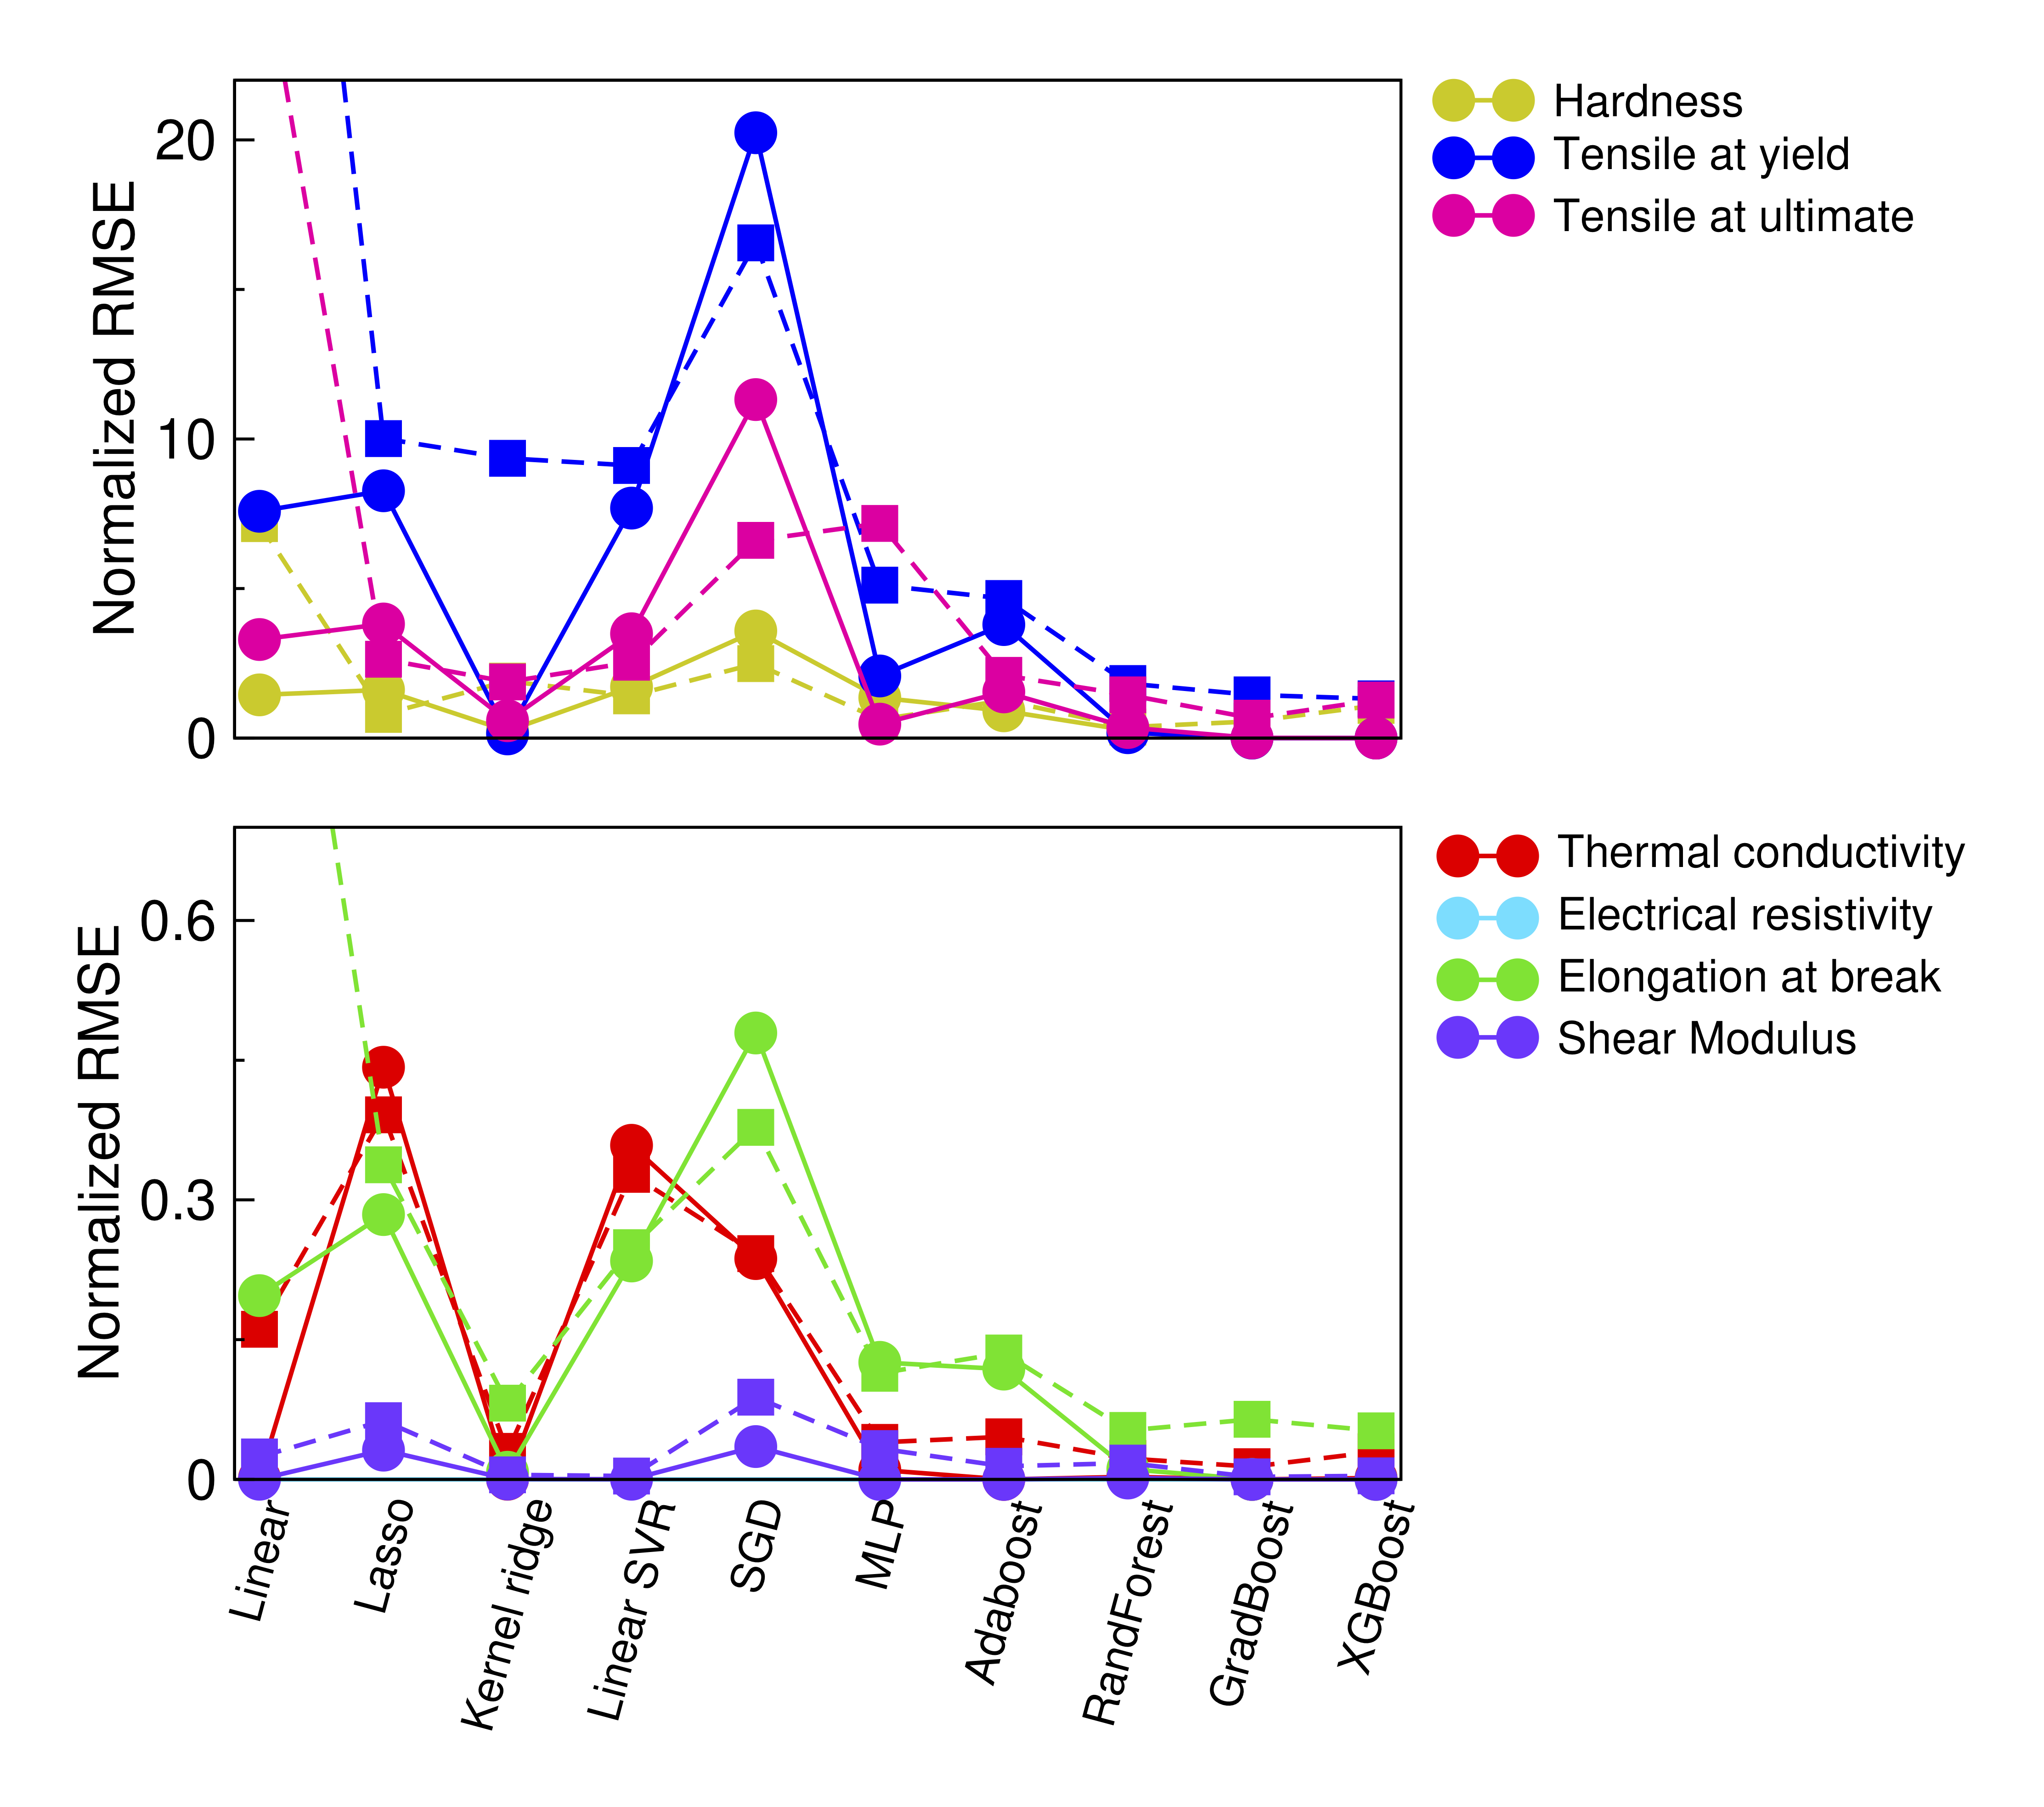
\includegraphics[width=0.95\linewidth]{figures/benchmark.png}
 \vspace{-10pt}
  \caption{Normalized root mean square error (RMSE) of different machine learning algorithms in predicting various physical properties. Training errors are shown in circles and solid lines, test errors are in squares and dashed lines.}
  \label{fig:benchmark}
\end{figure}


The y-axis is the calculated root mean square error (RMSE) value divided by the difference in the target data. This normalization step is essential so as to directly compare the performance of different machine learning algorithms in predicting quantities at various scales. The \texttt{sklearn} built-in performance score is not used here.

Interestingly, some trends can be identified across different algorithms as well as physical properties. In general, linear regression, Lasso, linear SVR and SGD algorithms lead to larger variance in normalized RMSE, while the rest have relatively better performance. XGBoost algorithm exhibits the best performance among the 10 benchmarked methods.

The physical properties are divided into two panels due to different scales of RMSE. We find it hard to have a good prediction in hardness and tensile strength, but this is no coincidence. It is exciting to notice that from the correlation heatmap analysis, it is clear that hardness is strongly and positively correlated to tensile strengths. This may suggest that these quantities are related to some other factors not considered here, such as processing and microscopic structures. And we need to include the other important features in order to build better machine learning models.


\begin{table*}
\begin{ruledtabular}
\caption{Hyper-parameters used in different machine learning algorithms for grid search.\label{tab:hyperparam}}
\centering
\begin{tabular}{ccc}
\sffamily Algorithm & \sffamily Parameter & \sffamily Values \\
\hline
Linear Regression & default & default \\
\hline
Lasso & `alpha' & \{ 1E-4, 0.001, 0.01, 0.1, 1 \}\\
\hline
& `kernel' & \{`linear', `poly', `rbf', `sigmoid' \} \\
Kernel Ridge & `alpha' & \{ 1E-4, 1E-2, 0.1, 1 \} \\
& `gamma' & \{ 0.01, 0.1, 1, 10 \} \\
\hline
Linear SVR & `C' & \{ 1E-6, 1E-4, 0.1, 1 \} \\
& `loss' & \{ `epsilon\_insensitive', `squared\_epsilon\_insensitive'\} \\
\hline
SGD & `alpha' & \{1E-6, 1E-4, 0.01, 1 \} \\
& `penalty' & \{`l2', `l1', `elasticnet'\} \\
\hline
& `activation' & \{`logistic', `tanh', `relu'\} \\
MLP & `solver' & \{`lbfgs', `adam', `sgd'\} \\
& `learning\_rate' & \{`constant', `invscaling', `adaptive'\} \\
\hline
Adaboost & `n\_estimators' & \{10, 100, 1000\} \\
& `learning\_rate' & \{0.01, 0.1, 1, 10\} \\
\hline
& `n\_estimators' & \{10, 100, 1000\} \\
RandForest& `min\_weight\_fraction\_leaf' & \{0.0, 0.25, 0.5\} \\
& `max\_features' & \{`sqrt', `log2', None\} \\
\hline
& `n\_estimators' &  \{10, 100, 1000\}\\
GradBoost & `min\_weight\_fraction\_leaf' &  \{0.0, 0.25, 0.5\}\\
& `max\_feature' &  \{`sqrt', `log2', None\}\\
\hline
& `n\_estimators' &  \{10, 50, 100, 250, 500, 1000\}\\
& `learning\_rate' &  \{1E-4, 0.01, 0.05, 0.1, 0.2\}\\
XGBoost & `gamma' &  \{0, 0.1, 0.2, 0.3, 0.4\}\\
& `max\_depth' &  \{6\}\\
& `subsample' &  \{0.5, 0.75, 1\}\\
\end{tabular}
\end{ruledtabular}
\end{table*}

\subsection{predict composition-property relationship}

From the previous section we choose to use Extreme Gradient Boosting algorithm for further analysis on alloy steel composition-relationship problems.

\begin{figure}[h]
  \center
  \vspace{-1mm}
 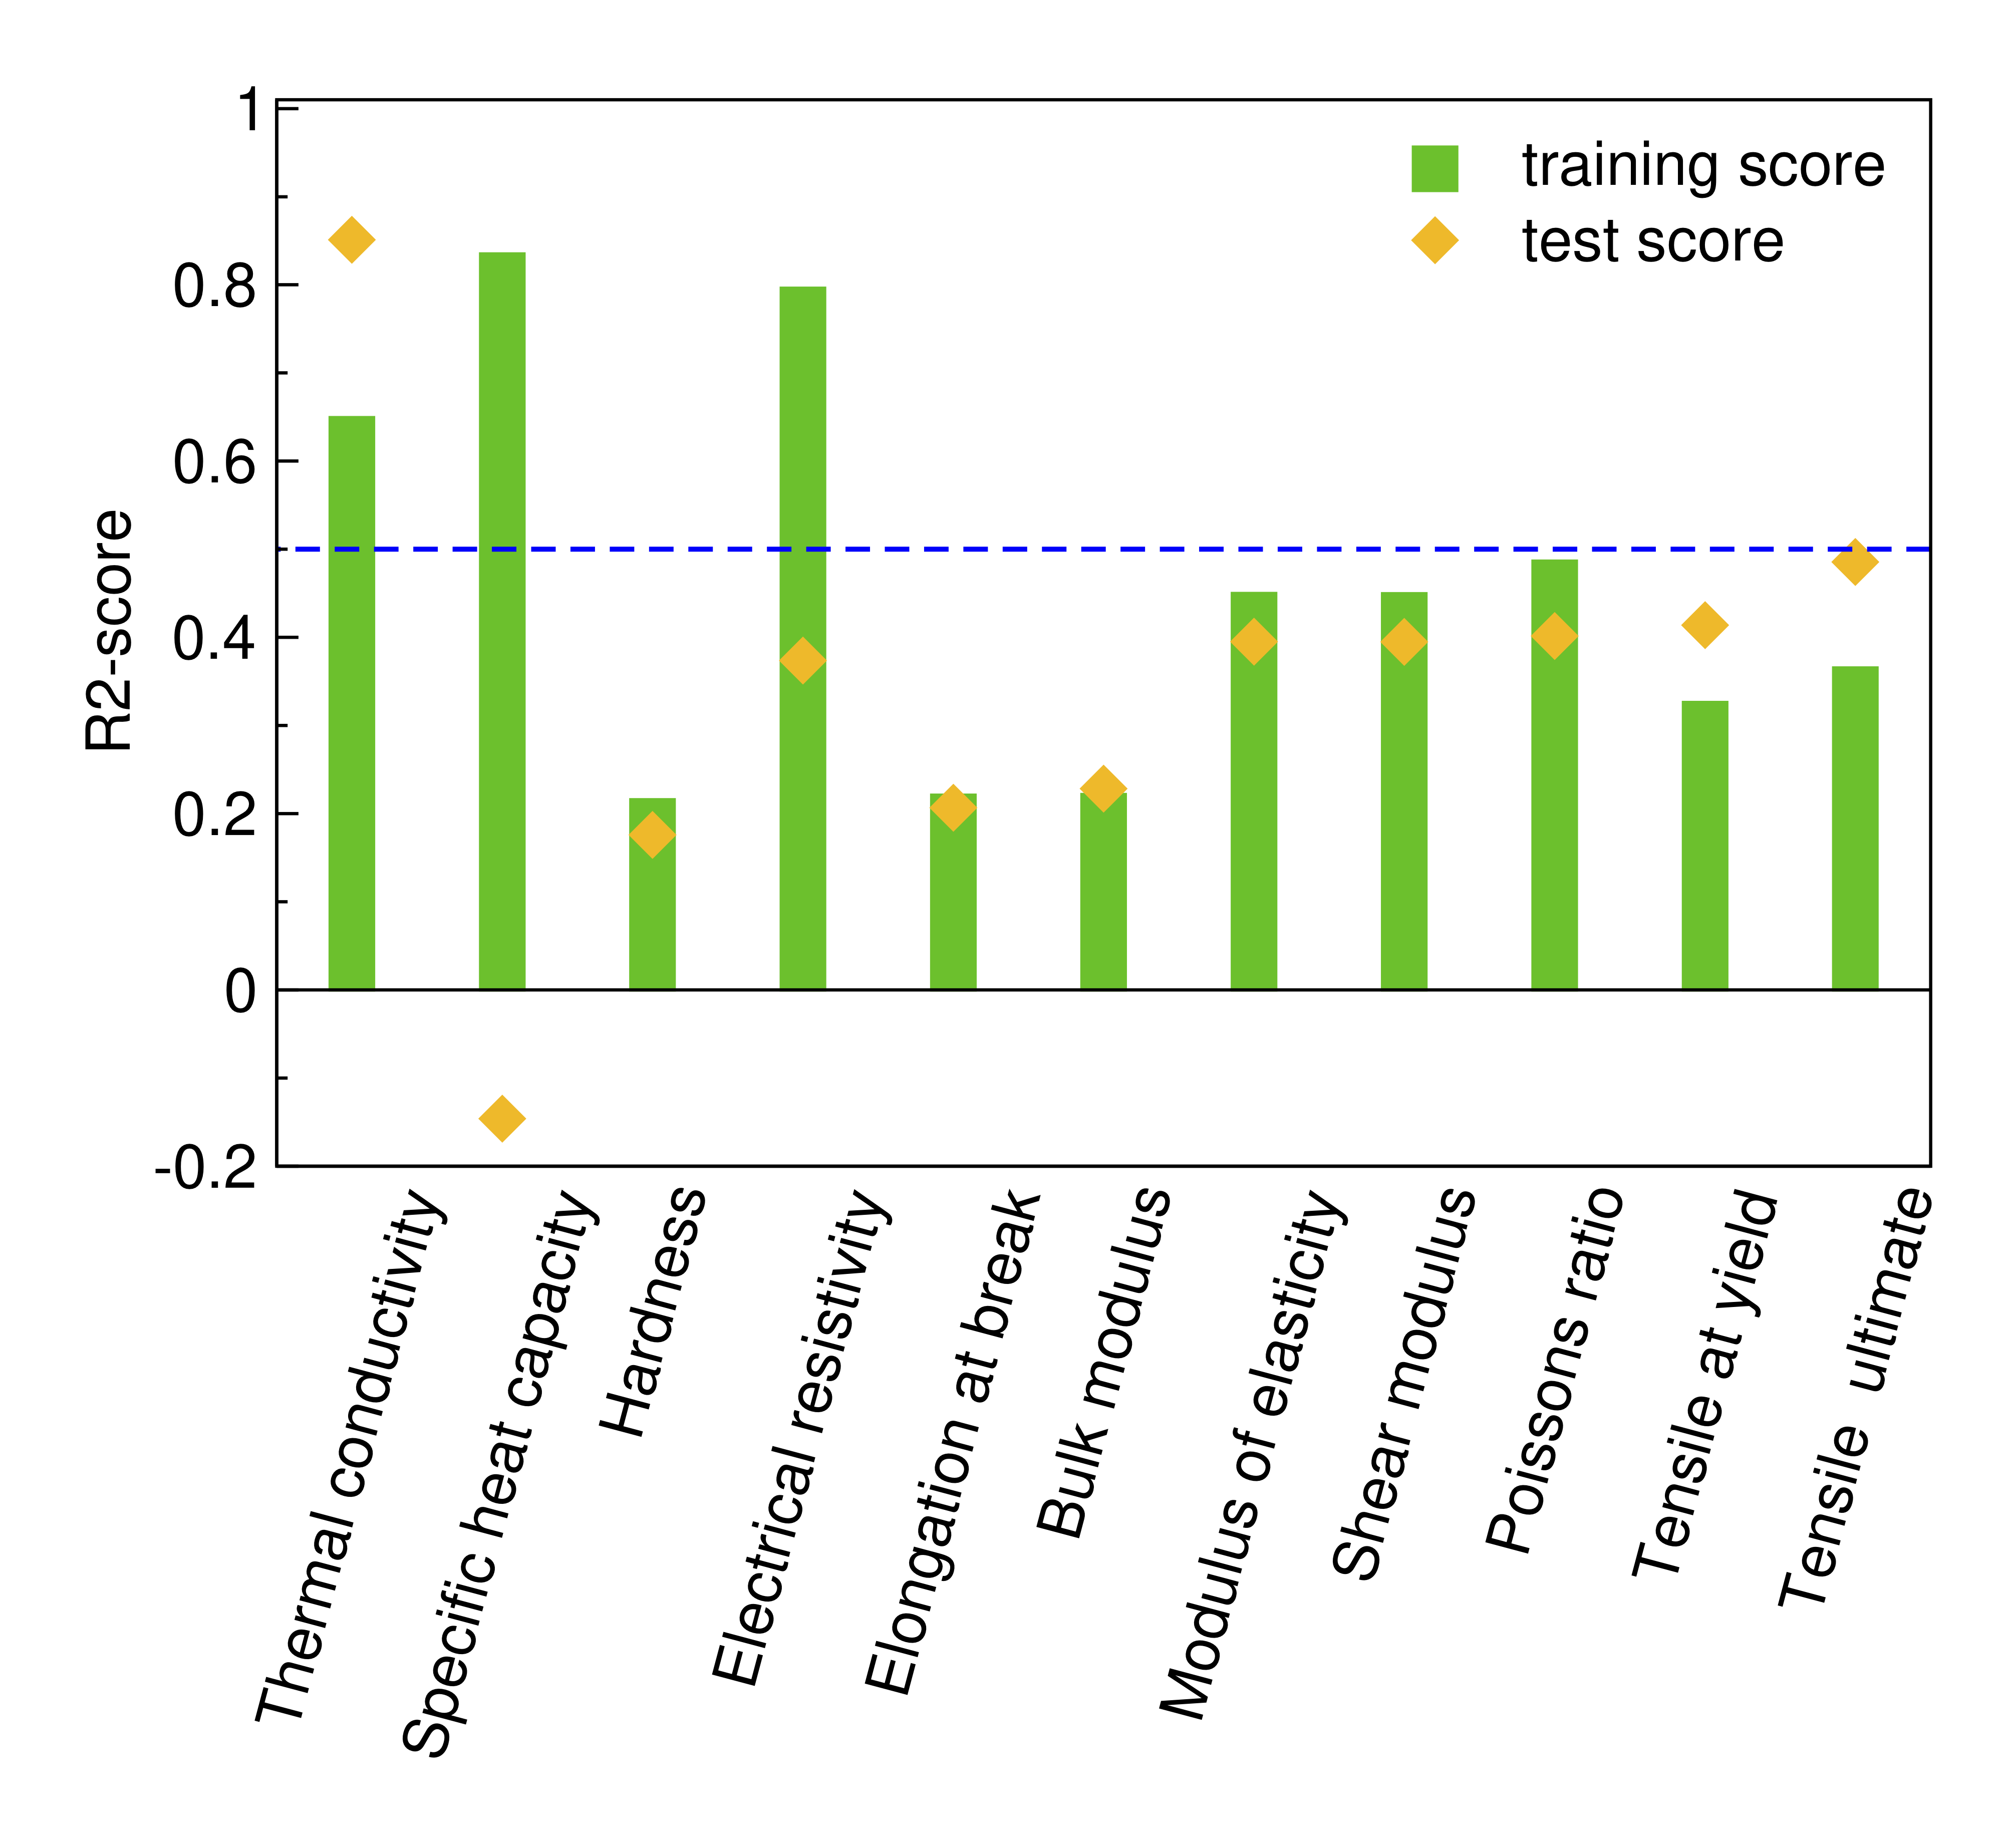
\includegraphics[width=0.95\linewidth]{figures/compo-prop.png}
  \caption{ADD CAPTION}
  \label{fig:compo-prop}
\end{figure}


\begin{figure}[h]
  \center
  \vspace{-1mm}
 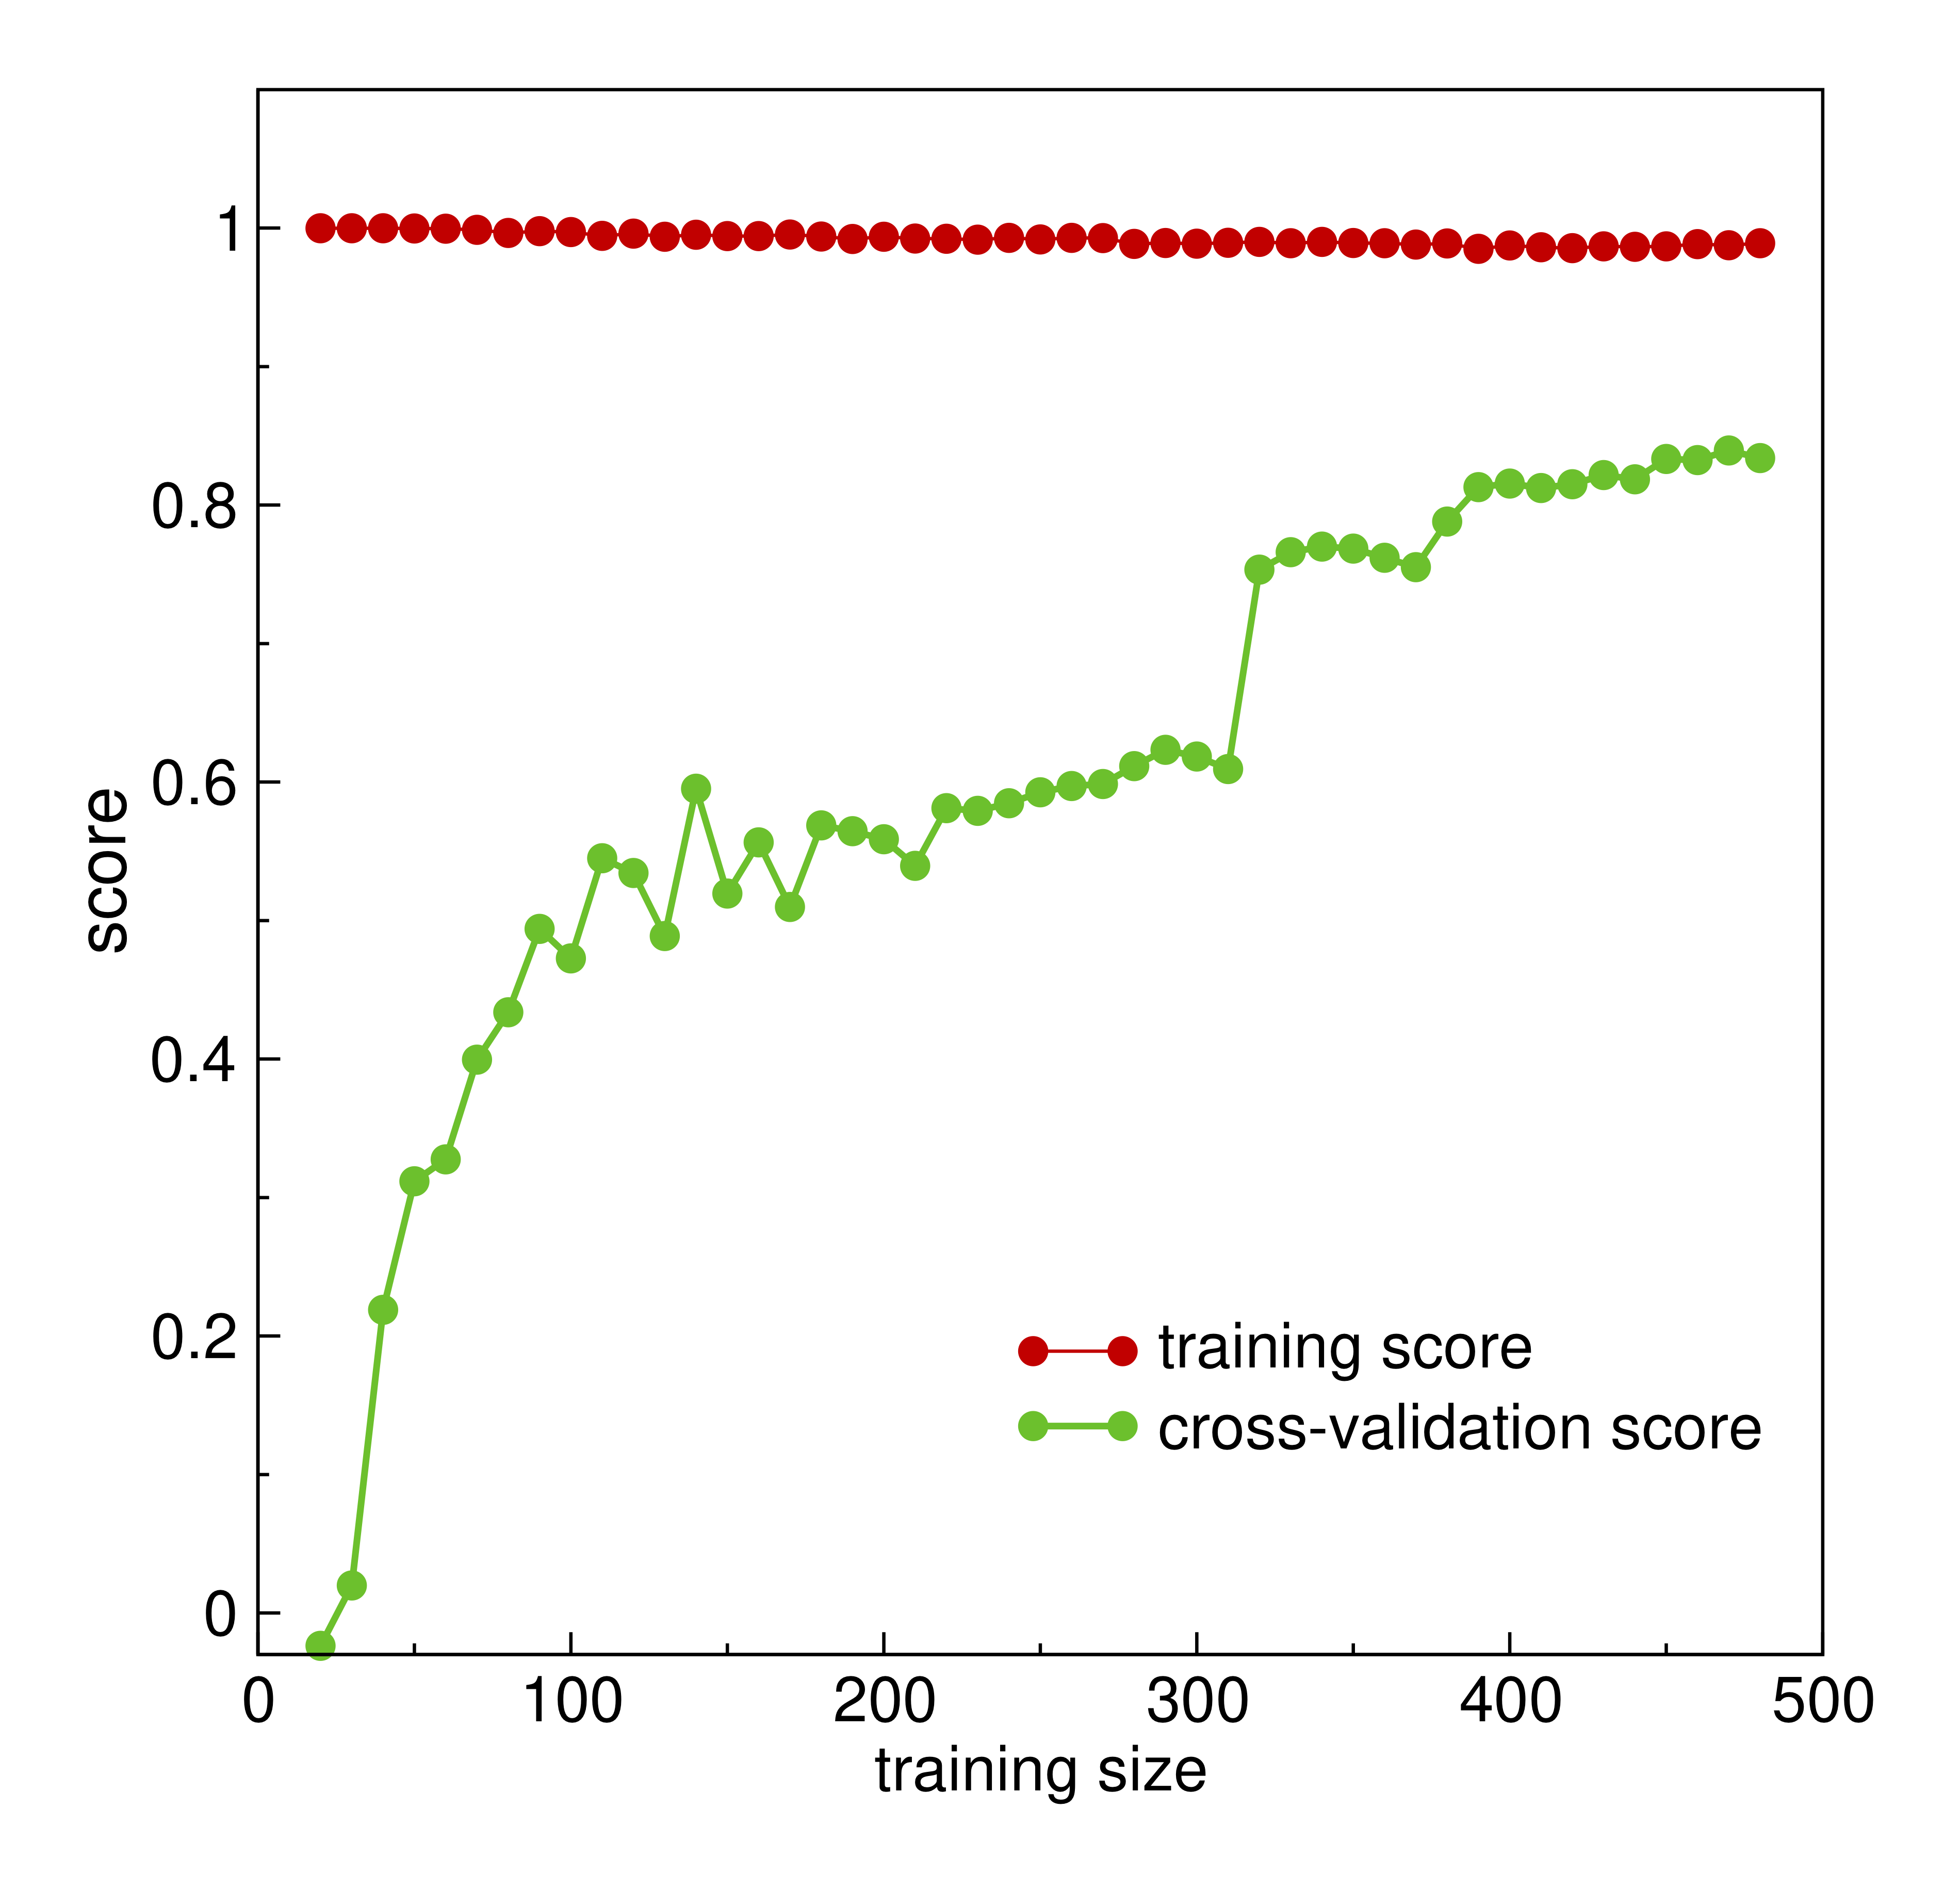
\includegraphics[width=0.95\linewidth]{figures/learning_curve.png}
  \caption{Learning curve of predicting thermal conductivity from chemical composition using XGBoost algorithm.}
  \label{fig:wyq4}
\end{figure}



%%%%%%%%%%%%%%%%%%%%%%%%%%%%%%%%%%%%
% CONCLUSIONS
%%%%%%%%%%%%%%%%%%%%%%%%%%%%%%%%%%%
\section{conclusions}



%\bibliography{reference.bib}

\end{document}



